\documentclass{extarticle}
\sloppy

%%%%%%%%%%%%%%%%%%%%%%%%%%%%%%%%%%%%%%%%%%%%%%%%%%%%%%%%%%%%%%%%%%%%%%
% PACKAGES            																						  %
%%%%%%%%%%%%%%%%%%%%%%%%%%%%%%%%%%%%%%%%%%%%%%%%%%%%%%%%%%%%%%%%%%%%%
\usepackage[10pt]{extsizes}
\usepackage{amsfonts}
\usepackage{amsthm}
\usepackage{amssymb}
\usepackage[shortlabels]{enumitem}
\usepackage{microtype} 
\usepackage{amsmath}
\usepackage{mathtools}
\usepackage{commath}
\usepackage[margin=1in]{geometry}
\usepackage{float}
\usepackage{cancel}
\usepackage{amsmath, amsfonts, amssymb}

%%%%%%%%%%%%%%%%%%%%%%%%%%%%%%%%%%%%%%%%%%%%%%%%%%%%%%%%%%%%%%%%%%%%%%
% PROBLEM ENVIRONMENT         																			           %
%%%%%%%%%%%%%%%%%%%%%%%%%%%%%%%%%%%%%%%%%%%%%%%%%%%%%%%%%%%%%%%%%%%%%
\usepackage{tcolorbox}
\tcbuselibrary{theorems, breakable, skins}
\newtcbtheorem{prob}% environment name
              {Problem}% Title text
  {enhanced, % tcolorbox styles
  attach boxed title to top left={xshift = 4mm, yshift=-2mm},
  colback=blue!5, colframe=black, colbacktitle=blue!3, coltitle=black,
  boxed title style={size=small,colframe=gray},
  fonttitle=\bfseries,
  separator sign none
  }%
  {} 
\newenvironment{problem}[1]{\begin{prob*}{#1}{}}{\end{prob*}}

%%%%%%%%%%%%%%%%%%%%%%%%%%%%%%%%%%%%%%%%%%%%%%%%%%%%%%%%%%%%%%%%%%%%%%
% THEOREMS/LEMMAS/ETC.         																			  %
%%%%%%%%%%%%%%%%%%%%%%%%%%%%%%%%%%%%%%%%%%%%%%%%%%%%%%%%%%%%%%%%%%%%%%
\newtheorem{thm}{Theorem}
\newtheorem*{thm-non}{Theorem}
\newtheorem{lemma}[thm]{Lemma}
\newtheorem{corollary}[thm]{Corollary}

%%%%%%%%%%%%%%%%%%%%%%%%%%%%%%%%%%%%%%%%%%%%%%%%%%%%%%%%%%%%%%%%%%%%%%
% MY COMMANDS   																						  %
%%%%%%%%%%%%%%%%%%%%%%%%%%%%%%%%%%%%%%%%%%%%%%%%%%%%%%%%%%%%%%%%%%%%%
\newcommand{\Z}{\mathbb{Z}}
\newcommand{\R}{\mathbb{R}}
\newcommand{\C}{\mathbb{C}}
\newcommand{\F}{\mathbb{F}}
\newcommand{\bigO}{\mathcal{O}}
\newcommand{\Real}{\mathcal{Re}}
\newcommand{\poly}{\mathcal{P}}
\newcommand{\mat}{\mathcal{M}}
\DeclareMathOperator{\Span}{span}
\newcommand{\Hom}{\mathcal{L}}
\DeclareMathOperator{\Null}{null}
\DeclareMathOperator{\Range}{range}
\newcommand{\defeq}{\vcentcolon=}
\newcommand{\restr}[1]{|_{#1}}


%%%%%%%%%%%%%%%%%%%%%%%%%%%%%%%%%%%%%%%%%%%%%%%%%%%%%%%%%%%%%%%%%%%%%%
% SECTION NUMBERING																				           %
%%%%%%%%%%%%%%%%%%%%%%%%%%%%%%%%%%%%%%%%%%%%%%%%%%%%%%%%%%%%%%%%%%%%%%
\renewcommand\thesection{\Alph{section}:}
\renewcommand\thesubsection{\Alph{section}.\arabic{subsection}}
\renewcommand\thesubsubsection{\Alph{section}.\arabic{subsection}.\arabic{subsubsection}}


%%%%%%%%%%%%%%%%%%%%%%%%%%%%%%%%%%%%%%%%%%%%%%%%%%%%%%%%%%%%%%%%%%%%%%
% DOCUMENT START              																			           %
%%%%%%%%%%%%%%%%%%%%%%%%%%%%%%%%%%%%%%%%%%%%%%%%%%%%%%%%%%%%%%%%%%%%%%
\title{\vspace{-2em}Chapter 9: IS-LM-PC Model}
\author{\emph{Summary}, by JF Viray}
\date{}

\begin{document}
\maketitle

\section{Putting the Philipps Curve (PC) in terms of Output ($Y$)}
Recall from the IS-LM model that the equations are in terms of output ($Y$) and the real interest rate ($r$). 
\begin{align*}
  \text{IS Relation: } Y &= C(Y-T) + I(Y, r + x) + G \\
  \text{LM Relation: } r &= \overline{r}
\end{align*}
From the previous chapter, we also have PC in terms of inflation and unemployment as:
$$\pi_t - \pi^e_t = -\alpha (u_t- u_n)$$

However, this creates a problem: the Phillips Curve is expressed in terms of inflation and unemployment, while the IS-LM model is in terms of interest rates and output. 
To bring them together, we need a link between unemployment and output, which we will describe right now. 
We can then rewrite the Phillips Curve so that IS, LM, and PC are all expressed with output ($Y$) as the common variable.

First, we assume a production function $Y = AN$ where $A$ represents productivity and $N$ is the number of employed. To make our lives simpler, we let $A = 1$, so output is directly proportional to how many workers there are, that is, $$Y = N$$.

This should make sense since everyone who is employed ($N$) will be part of production ($Y$).
We then use our definition of the unemployment rate where $u = \frac{U}{L}$ such that $L = U + N$. Then, $N = L - U = L - L \cdot u =  L(1 - u)$. We thus now have our relationship between output and unemployment as:
$$Y = L(1-u)$$
When the economy is at the natural rate of unemployment, we say that it operates at potential output \(Y_n\), given by $ Y_n = L(1 - u_n).$ 
Notice that the output gap $(Y_t - Y_n)$ is inversely related to the unemployment gap \((u_t - u_n)\) as shown below:

\begin{align*}
    Y_t - Y_n &= L(1-u_t) - L(1-u_n) \\
    \implies \quad \quad \quad \; \: Y_t - Y_n &= L - L \cdot u_t - L + L \cdot u_n \\
    \implies \quad \quad \quad \; \: Y_t - Y_n &= - L \cdot u_t + L \cdot u_n \\
    \implies \quad \quad \quad \; \: Y_t - Y_n &= -L (u_t - u_n) \\
    \implies \quad -\frac{1}{L}(Y_t - Y_n) &= u_t - u_n
\end{align*}

Starting with our original Phillips Curve,  


$$\pi_t - \pi^e_t = -\alpha (u_t - u_n),$$

we use the relationship between the unemployment gap and the output gap of $ -\frac{1}{L}(Y_t - Y_n) = u_t - u_n$. This gives  

$$\pi_t - \pi^e_t = \frac{\alpha}{L}(Y_t - Y_n).$$

We now have a chain of implication that all begins in the labor market where if unemployment is below its natural rate, output will also be above its potential. In addition to this, inflation will rise above the expected inflation. 
Note that since expectations for inflation have been achored recently (from the years 2000s onwards), we denote expected inflation as its historical average ($\pi_t^e = \overline{\pi}$). 
\begin{enumerate}
  \item $Y_t > Y_n \implies \pi_t > \overline{\pi}$ 
  \item $Y_t < Y_n \implies \pi_t < \overline{\pi}$
  \item $Y_t = Y_n \implies \pi_t = \overline{\pi} $
\end{enumerate}



\section{Actually Using the IS-LM-PC Model}

\begin{figure}[H] 
  \centering % Left side: image 
  \begin{minipage}{0.4\linewidth} 
    \centering 
    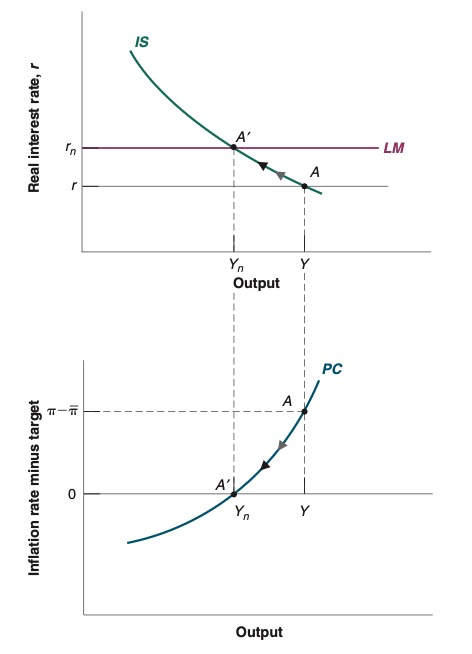
\includegraphics[width=\linewidth]{IS-LM-PC.png} 
    \caption{The IS-LM-PC Model} 
    \label{fig:IS-LM-PC} 
  \end{minipage}% 
  % Right side: text 
  \begin{minipage}{0.6\linewidth} 
    IS-LM model talks about how the real interest rate affects output.  Then, from the Philipps Curve, it talks how output affects inflation. Now, this will be kind of hard since we have two graphs to represent the three markets, so we'll take it slowly.

    \vspace{2mm}

    To make sense of Figure \ref{fig:IS-LM-PC}, think of the top graph as showing the goods and money markets together through the IS-LM framework. 
    The horizontal axis is output $Y$ and the vertical axis is the real interest rate $r$. The intersection of IS and LM determines the short-run equilibrium output $Y$ for a given $r$.

    \vspace{2mm}

    The bottom graph shows the Phillips Curve, talks about the labor market. However, we manipulated it so much in section $A$ that we eventually have a relationship between output to inflation. 
    Here, the horizontal axis is again output $Y$, and the vertical axis is inflation rate MINUS target $(\pi - \overline{\pi})$. We now have to delineate when the output and inflation gaps are positive or negative. We do this by having an auxillary line in the $y$-axis to determine when inflation meets target, that is, $\pi - \overline{\pi} = 0$.
    
    \vspace{2mm}
    By connecting the two graphs conceptually:
    \begin{enumerate}
        \item Start with the IS-LM model. We started at point $A$ which has a given real interest rate $r$ with the corresponding short-run output $Y$.
        \item Go downwards to the graph for the Phillips Curve to translate that short-run $Y$. We see that there is a positive output gap from $Y > Y_n \implies Y - Y_n > 0$, which has a corresponding positive inflation gap $\pi - \overline{\pi} > 0$.
        \item If $Y \neq Y_n$, a positive or negative output gap exists. The economy would start having inflation that the central bank DOES NOT WANT. As such, it will do its montery policy to make sure that inflaion goes back to target.
    \end{enumerate}
  \end{minipage} 
\end{figure}

In the medium run, the adjustment of the real interest rate ensures that output returns to its natural level $Y_n$, unemployment returns to $u_n$, and inflation converges to the target $\pi^*$. 
At this point, the interest rate and money growth adjust to sustain the equilibrium. Because the goods, financial, and labor markets are all in balance, monetary policy no longer affects real variables in the medium run. This property is called the neutrality of money.


\section{Playing with the IS-LM-PC Model}
\subsection{Zero Lower Bound and Deflation Spirals}
\begin{figure}[H] 
  \centering % Left side: image 
  \begin{minipage}{0.35\linewidth} 
    \centering 
    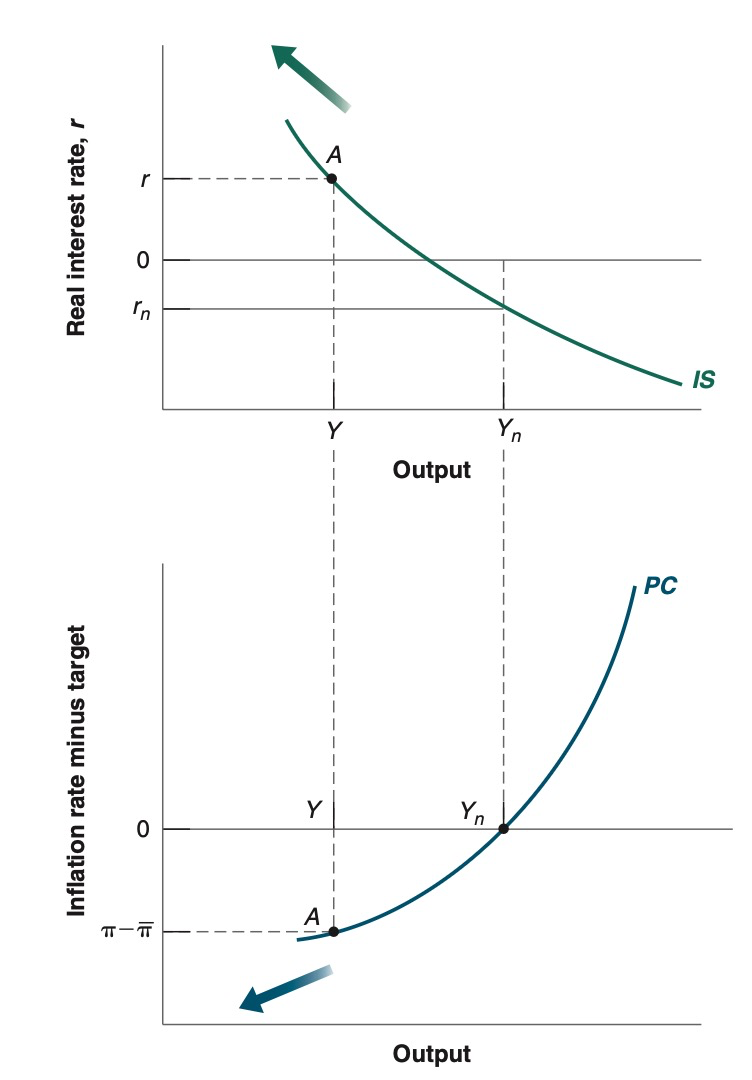
\includegraphics[width=\linewidth]{deflation.png} 
    \caption{Deflation Spiral} 
    \label{fig:deflation} 
  \end{minipage}% 
  % Right side: text 
  \begin{minipage}{0.65\linewidth}
    Suppose the economy is stuck in a recession and we are at point A. Output is some $Y$ with its corresponding real interest rate $r$. From the way the Figure 2 is drawn, suppose the natural real interest rate $r_n$ is negative.

    \vspace{2mm}
    From the IS-LM model, we go down to the Philipps Curve and see output is below potential ($Y - Y_n > 0$) and thus have a corresponding negative inflation gap ($\pi - \overline{\pi}$). The inflation gap may be so negative that we are experiencing deflation, so $\pi < 0$ is a possibility. Let us assume that the we are in deflation right now.
    
    \vspace{2mm}
    Recall that the nominal interest rate cannot go below zero, and we have a relation between the real interest rate, nominal interest rate, and inflation of $r = i - \pi$. Given our scenario right now, the central bank is doing its monetary policy and set $i = 0$. However, we have assumed deflation, so $\pi < 0$. Then the lowest possible value of the real interest rate is a positive number. This is shown as $r = i - \pi = 0 - \pi = -\pi > 0$. 

    \vspace{2mm}
    Here is the problem: with deflation ($\pi < 0$) and the zero lower bound ($i = 0$), the real interest rate is $r = i - \pi = -\pi > 0$. So even if the central bank wants $r_n < 0$, it cannot achieve it. 
    This constraint can cause expectations to shift, activating the accelerationist Phillips Curve and pushing the economy into a deflationary spiral.

  \end{minipage} 
\end{figure}

\subsection{Fiscal Consolidation}
\begin{figure}[H] 
  \centering % Left side: image 
  \begin{minipage}{0.35\linewidth} 
    \centering 
    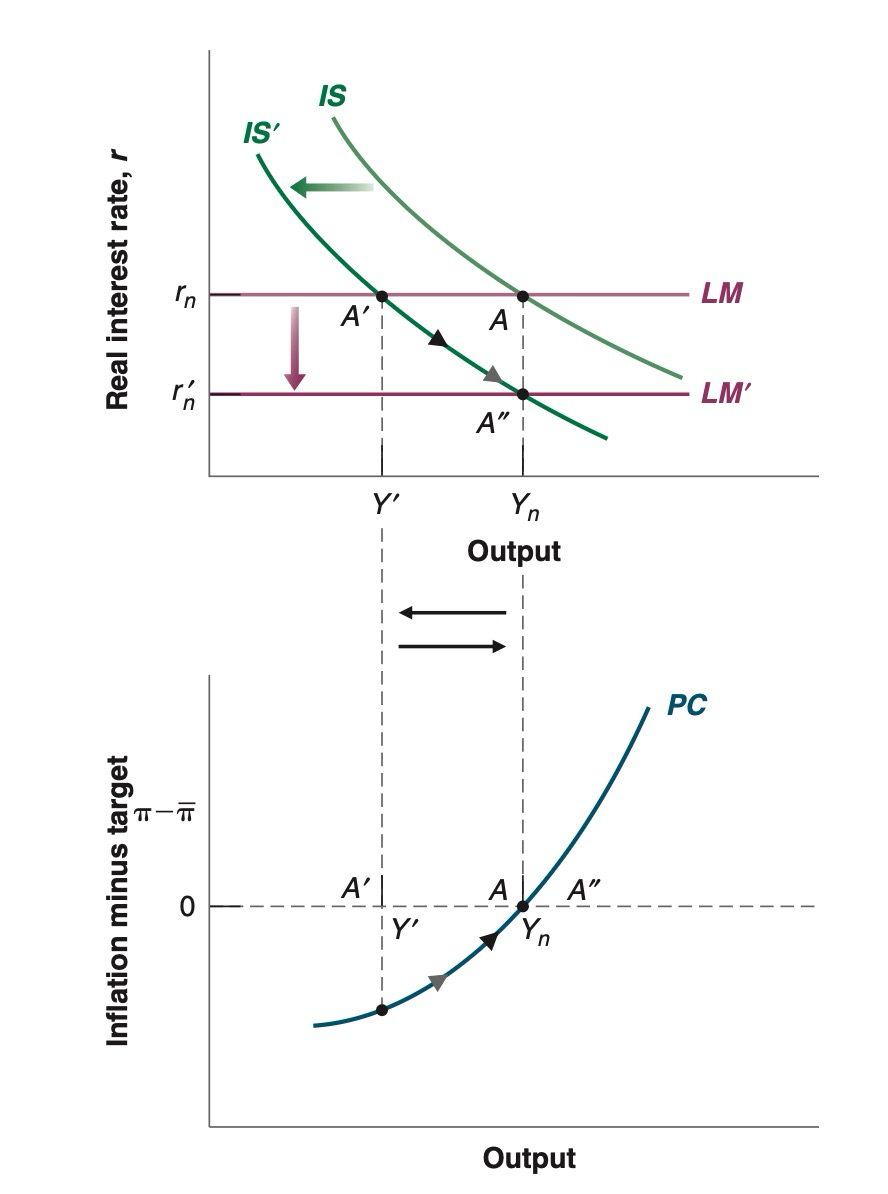
\includegraphics[width=\linewidth]{fiscal consolidation.png}
    \caption{Fiscal Consolidation} 
    \label{fig:deflation} 
  \end{minipage}% 
  % Right side: text 
  \begin{minipage}{0.65\linewidth}
    Going from point $A$ to $A'$ and from $A'$ to $A''$, the process is to first look at IS-LM model and then the PC part. We provide the chain of implication below as a summary.
\begin{center}
\text{Point A to A'} \\
$\Delta T^+ \;\implies\; \Delta C^- \;\implies\; \Delta Y^- \;\implies\; Y - Y_n < 0 \;\implies\; \pi - \overline{\pi} < 0$ 
\end{center}

\begin{center}
\text{Point A' to A''} \\
$\Delta r_n^- \;\implies\; I^+ \;\implies\; \Delta Y^+ \;\implies\; Y - Y_n = 0 \;\implies\; \pi = \overline{\pi}$ 
\end{center}

Let us suppose that we are in the equilibrium of the middle run, so we start at point A. Then, the government wants to do fiscal consolidation, so they increase taxes. Then, disposable income decreases and thus consumption and output must also decrease. The IS curve shifts to the left, and now the economy is operating at point $A'$. If we go down to the Philipps Curve, we see that we are below potential, so we would also have a negative inflation gap. We have now shown how the economy moved from point $A$ to $A'$.
\vspace{2mm}

Let us now see how the economy moves from point $A'$ to $A''$. Because inflation is below target, the central bank does not like that fact. They will decrease the interesst rate so that investment increases and thus output goes back to potential. Because output is at potential, inflation is also back to the central bank's target. 
Notice however that the OVERALL change from point $A$ to $A''$, output remained constant by consumption decreasing and investment increasing.
  \end{minipage} 
\end{figure}

\subsection{Effects of an Increase in the Price of Oil}


\begin{figure}[H] 
  \centering % Left side: image 
  \begin{minipage}{0.35\linewidth} 
    \centering 
    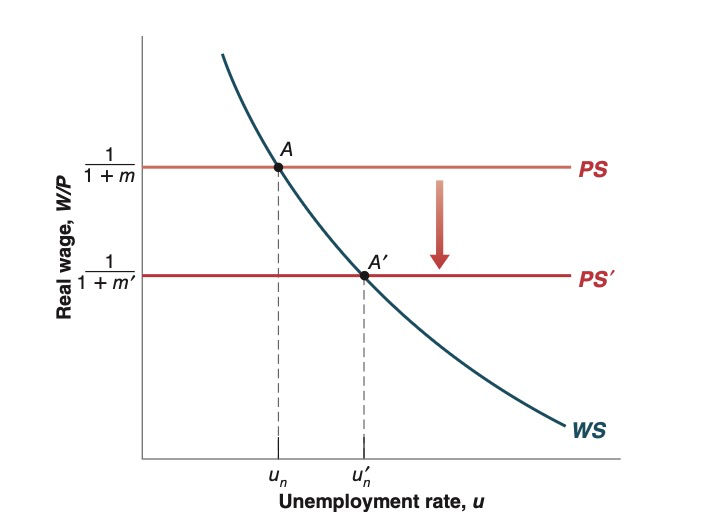
\includegraphics[width=\linewidth]{labor.png} 
    \caption{Labor Market} 
    \label{fig:labor} 
  \end{minipage}% 
  % Right side: text 
  \begin{minipage}{0.65\linewidth}
    For this chapter, we usually start with the IS-LM model. However, this one is going to be a doozy since we actually start with the Philipps Curve. 
    
    \vspace{2mm}
    
    Let us suppose there is an increase in the price of oil, which we will treat as higher markup $m$ because it raises firms’s non-wage costs. 
    From Chapter 8, the easiest way to model the increase of a non-wage cost is to increase the markup $m$. 
    We then turn to the labor market where the increase in the markup from $m$ to $m'$ shifts the Price-Setting (PS) curve downward, raising the natural rate of unemployment from $u_n$ to $u_n'$ as shown in Figure \ref{fig:labor}. 
  \end{minipage} 
\end{figure}


We now return to the IS-LM-PC model. Suppose the initial equilibrium is at point $A$ in both the goods and finiancial markets (top panel) and labor market (bottom panel), as shown in Figure 5. 
Thus, output is at potential ($Y = Y_n$); inflation is at target, and the real interest rate is equal to $r_n$. When the price of oil increases, potential output falls from $Y_n$ to $Y_n'$, shifting the PC curve up from PC to PC. 
If the IS curve stays fixed and the central bank holds the real rate constant, output remains the same, but inflation rises above target. The short-run equilibrium is at point $A'$.

\begin{figure}[H]
    \centering 
    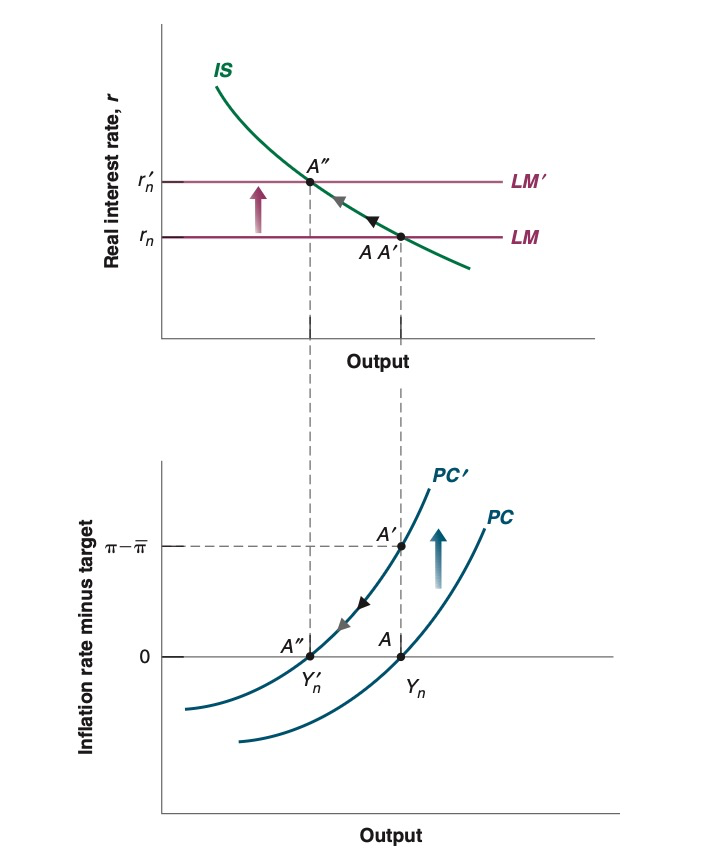
\includegraphics[width=0.45\linewidth]{stagflation.png}
    \caption{Effects on the Increase of the Price of Oil} 
    \label{fig:oil} 
\end{figure}


If the central bank leaves the real rate unchanged, output continues to exceed the new lower potential, inflation stays high, and expectations drift upward, leading to accelerating inflation. To prevent this, the central bank must raise the real rate. 
The economy then moves from A9 to A0 along the IS curve (top panel) and from A0 to A0 along the PC curve (bottom panel). Output falls to its new lower level, and inflation returns to target. In the medium run, the economy settles at A0, with permanently lower potential output. 
This adjustment path combines lower output with above-target inflation—a situation known as stagflation.
\end{document}